%%%%%%%%%%%%%%%%%%%%%%%%%%%%%%%%%%%%%%%%%%
%
% Cosecivi 2017
% http://gaia.fdi.ucm.es/sites/cosecivi17
% 12 pages max
%
%%%%%%%%%%%%%%%%%%%%%%%%%%%%%%%%%%%%%%%%%%

\documentclass{llncs}

\usepackage{float}
\usepackage[english]{babel}
\usepackage[utf8]{inputenc}
\usepackage{epsfig}
\usepackage{graphicx}
\usepackage{subcaption}
\captionsetup{compatibility=false}
\usepackage{color}
\usepackage{amsfonts}
\usepackage{amsmath}
%\usepackage{mathabx}
\usepackage{hyperref}
\usepackage{listings}

%\usepackage{hyperref}
%\usepackage{subfigure}
%\usepackage[colorinlistoftodos, textwidth=3.2cm, shadow]{todonotes}

%\usepackage{algorithm}
%\usepackage{fixltx2e}
%\usepackage{algpseudocode}

\usepackage{multirow}

% To use Call inside another Call (algorithms)
%\MakeRobust{\Call}

\graphicspath{{images/}}

\newcommand{\pacman}{Ms. Pac-Man vs. Ghosts }
\newcommand{\paco}{Pac-Man }
\newcommand\tab[1][1cm]{\hspace*{#1}}
\newcommand\menostab[1][-0.5cm]{\hspace*{#1}}

%%%%%%%%%%%%%%%%%%%%%%%%%%%%%%%%%%%%%%%%%%
%
% Title
%
%%%%%%%%%%%%%%%%%%%%%%%%%%%%%%%%%%%%%%%%%%
\title{Title\thanks{Supported by Spanish Ministry of Economy and Competitiveness under grants TIN2014-55006-R and TIN2014-57028-R}
}

\author{Héctor Laria Mantecón, Jorge Sánchez Cremades, José Miguel Tajuelo Garrigós, Jorge Vieira Luna, Carlos Cervigon Rückauer, Antonio A. S\'{a}nchez-Ruiz}

\institute{
	Dep. Ingenier\'{\i}a del Software e Inteligencia Artificial \\
	Universidad Complutense de Madrid (Spain) \\
	\email{\{hlaria, jorsan06, jtajuelo, jovieira, ccervigon, antsanch\}@ucm.es}
}

\begin{document}

\maketitle
%%%%%%%%%%%%%%%%%%%%%%%%%%%%%%%%%%%%%%%%%%
%
% Abstract
%
%%%%%%%%%%%%%%%%%%%%%%%%%%%%%%%%%%%%%%%%%%
\begin{abstract}
In this work we study Ms. Pac-Man vs Ghosts bot development using gramatical evolution. We make use of derivation trees to represent programs that Pac-Man runs to play. The programs are encoded as an array of codons, which are evolved using a grammatical evolution algorithm.
When a program is produced from its grammar, we need to execute it in the game for evaluation. We do that parsing the code and generating a game tree. For the Pac-Man controller to query a movement from that tree every turn, all it has to do is navigate the tree from the root down to a terminal node.

We will be using "medium level" and "high level" grammars, the first using calls to a set of functions that extract raw information from the game, the latter using more complex functions created by us that mix raw information with expert-knowledge. 

To make the evolution process more efficient, we perform a series of optimizations to the evolutionary algorithm. These include running parallel evaluations to save time, and creating multi-objective fitness functions to better guide the evolution process. We will be exploring the results of multi-objective optimization in detail.

\keywords{Genetic programming, grammatical evolution, multi-objetive optimization, Pac-Man, reactive artificial intelligence, decision trees, {\color{red}bots in video-games?}}
\end{abstract}

%%%%%%%%%%%%%%%%%%%%%%%%%%%%%%%%%%%%%%%%%%
%
\section{Introduction}
\label{sec:intro}
%
%%%%%%%%%%%%%%%%%%%%%%%%%%%%%%%%%%%%%%%%%%

{\color{red}Dejar para el final}

%%%%%%%%%%%%%%%%%%%%%%%%%%%%%%%%%%%%%%%%%%
%
\section{Related Work}
\label{sec:relatedWork}
%
%%%%%%%%%%%%%%%%%%%%%%%%%%%%%%%%%%%%%%%%%%

\subsection{Genetic Programming}
Genetic Programming is one of the many different branches of algorithms that exist inside Evolutionary Algorithms. \cite{poli_langdon_mcphee_koza_2008}
Genetic Programming tries to produce the best program, in a determined programming language, using an Evolutionary Algorithm approach. The programs are encoded using trees (genome)  in which each node represents a token of the chosen programming language, hence each individual of the population is a program which will be selected, crossover and mutated using different selection, crossover and mutation operators and his genome will be transformed into the final program (phenotype) and will be evaluated. This process is repeated several times and the final solution will be the individual with the program with the best score of the whole population.\cite{cervigon}
Genetic Programming main drawback is that the use of trees to encode the genome is very heavy in terms of memory, specially when bloating occurs.\cite{Poli2003}

Genetic Programming has been used previously to evolve Artificial Intelligence controllers, concretely, Koza\cite{koza1992genetic} used a Genetic Programming approach for developing a controller for the Pac-Man character of a custom version of the game. He used a set of high level operators for maze information retrieval (\textit{DISF - Distance to Fruit}) and Pac-Man direct control (\textit{AFRUIT - Advance to Fruit}).
More work about Artificial Intelligence in Pac-Man using Genetic Programming has been made, Alhejali and Lucas\cite{alhejali_lucas_2010}
also used high level operators with some of them even more abstract (\textit{isInDanger(takes two arguments), IsToEnergizerSafe(takes two arguments) or toSafety}) while Brandstetter and Ahmadi\cite{brandstetter_ahmadi_2012}
used low level action operators for Pac-Man movement (\textit{UP, DOWN...}), obtaining better results in points compared with the previous controllers.
\subsection{Grammatical Evolution}
Grammatical Evolution is similar to Genetic Programming in that both evolve programs to find the best one but the encoding of the programs (genotype) in Grammatical Evolution is different. Now, the genotype is an array of integers where each integer represents the rule of a grammar, written in Backus-Naur Form,
that will be chosen to produce the program (phenotype) when the genotype is decoded. So now the process of crossover and mutation is done with the array, increasing performance in time and memory and thanks to BNFs languages are very easy to design and change without reimplementing or modifying the algorithm code.\cite{o'neill_ryan_2012}

With this new representation of the genotype classical crossover operators, like the single-point crossover, and classical mutation operators, like integer flip mutation, work relatively good but they produce too much noise in the phenotype, specially crossover which generates chaotic populations so new operators had been developed to try to avoid this destructive behaviour. This new developed operators produce better results than the classical ones like LHS replacement crossover, which tries to do the crossover less destructive by taking into account the phenotype structure and not just the genotype \cite{harper_blair_2005}
and Neutral Mutation for improving population's diversity.\cite{oesch_maringer_2014}

As Genetic Programming (GP), Grammatical Evolution (GE) has been previously used to evolve a Pac-Man controller. Galván-López, Swafford, et al.\cite{galvan2010evolving}
developed a similar approach to Koza's GP approach, they used high level operators for Pac-Man movement (ANG - Avoid Nearest Ghost) and information retrieval (avgDistBetGhosts). This operators are terminal symbols of a BNF developed by them, which has if-else statements to achieve determined outputs based on some conditions processed by the if statement. These conditions are of the form (<var><comparison><var>) where <var> could be a number or an information retrieval operator and <comparison> an inequality symbol. With this approach they achieved similar results to GP controllers with the advantage that the BNF could be changed easily changing adding restrictions or features easily.

Other interesting study for evolving Pac-Man controllers with GE was made by Liberatore, Mora, et al.\cite{Liberatore2014}
They used GE with Flocking Strategies to develop a Swarm-type intelligent for the Pac-Man Ghosts controllers. This approach was able to model complex behaviours for the Ghosts, making them more challenging to beat.

We use the \paco implementation described in section 3 as our starting point, integrated with JECO (\textit{Java Evolutionary COmputation library}) \cite{jecorepo}. JECO is a framework which supports different evolutionary computation techniques, including what we wanted to try in \paco: Simple and multi-objective grammatical evolution.
%%%%%%%%%%%%%%%%%%%%%%%%%%%%%%%%%%%%%%%%%%
%
\section{\pacman AI}
\label{sec:pacmanai}
%
%%%%%%%%%%%%%%%%%%%%%%%%%%%%%%%%%%%%%%%%%%


\begin{figure}[H]
	\centering
	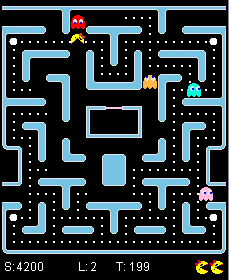
\includegraphics[width=8cm]{images/PacMan_ss.png}
\end{figure}


\subsection{The game}

In the version of the game we use\cite{mspacmangithub} there is a set of four pre-generated toroidal 2D labyrinths, in which the ghosts and \paco move. The ghosts always start in the "Lair", a rectangle in the middle of the map in which \paco cannot enter. \paco starts in the bottom of the map.

Each labyrinth is composed of corridors and junctions filled with a lot of pills and four power pills. Both give points to \paco as he walks over them, and power pills make him able to eat the ghosts for a short period of time, while also slowing them. Eating ghosts will give \paco points, earning some extra ones if he eats various ghosts in a row during the same power pill buff duration.

\paco will try to eat all the pills and power pills to advance levels, while avoiding the ghosts, which will try to hunt him, making him lose a live when they walk over him. A level is completed when there are no pills or power pills left, and there are an infinite number of levels, repeating the same set of 4 labyrinths consecutively.

\paco will strive to eat all the pills and power pills in the map to advance levels, while trying to get as much points as possible eating any ghosts he can, since each 10.000 points achieved he gets an extra life.

The game ends either when \paco loses his three lives or after 24.000 turns, considering a turn passes every time both \paco and the ghosts make a movement.

\subsection{Bot implementation architecture}

Both the ghosts and \paco use controllers to determine which movement is the best to make every turn. These controllers are the ones that must be implemented to participate in the competitions, which can be done using any technique available.

Every turn the game provides the controllers with its current state, so that the controller can seek relevant information it needs to choose a movement. Such information includes the pre-calculated distance from a point of the map to another (useful to check distances between \paco and the ghosts), which is the movement that puts you further away from any other position (useful to run away from the ghosts), which movements are possible given a position, testing if a position is a junction or not, etc. 

We've greatly increased the information to obtain by combining those given functions, like getting a movement towards the closest junction, the closest edible ghost, or the closest power pill.

The original code also comes with various examples of controllers like random movements for \paco and the ghosts, aggressive behavioured ghosts, or a basic one for \paco that takes into account if the surrounding ghosts are edible or not.

\subsection{Previous competitions}

\paco has been used in many bot implementing competitions, of which the most important are:

\begin{itemize}
\setlength{\itemindent}{-.3cm}
\item "Ms Pac-Man Competition"\cite{mspacmancompetitionwebsite}

This competition took place six times between 2007 and 2011. It used a different architecture to ours in which the participants had to capture the screen of the game to obtain game status information. 
\item "Ms. Pac-Man Vs. Ghost Team Competition"\cite{pacmanvsghostsaiwebsite}

Currently active, this competition was held in CIG 2016\cite{pmvsghostspaper2016} and is to be held again in 2017. It uses our same base architecture, although in their implementation the visibility of the agents is limited by "Partial Observability", in which both \paco and the ghosts can only obtain information of the game that is in their line of sight, this is, the corridor they are in or, if they are in a junction, the corridors that cross that junction.
\end{itemize}


%%%%%%%%%%%%%%%%%%%%%%%%%%%%%%%%%%%%%%%%%%
%
\section{A bot based on grammatical evolution}
\label{sec:sec1}
%
%%%%%%%%%%%%%%%%%%%%%%%%%%%%%%%%%%%%%%%%%%

\subsection{General idea}

The general idea is taking a Grammatical Evolution approach in order to generate \paco controller codes, which play automatically the game. This generated codes (the solutions) belong to the language generated by a user defined context-free grammar, more precisely a Backus-Naur Form denoted grammar.\cite{o'neill_ryan_2012} 

By using Grammatical evolution we were able to reduce and refine the search space the evolutionary algorithm will explore, deciding to generate only Reactive Artificial Intelligence based bots. This type of Artificial Intelligence first evaluates the world and then executes and actions, following in our case condition-action rules defined by the grammar. This way, we expect to produce simple programs, which will not be able to encode explicitly advanced strategies consisting of action sequences.

For example, one of the results of the Grammatical Evolution is the code \texttt{if(distClosNEGhost>10)\{toClosP\} else\{awayClosNEGhost\}}. This bot checks every turn if the distance to the closest non edible ghost is lower than 10. In that case, \paco will try to escape from the ghost. Otherwise, \paco will move towards the closest pill.

This code is implemented using a decision tree, using branch nodes for game state evaluations and leaf nodes for specific actions.


\subsection{Grammar design}

In order to allow our bot to interact with the game, we had to create two categories of methods:

\subsubsection{Actions}
Methods which result in a move for the bot to execute. For example:\newline

\menostab\textit{distClosPill} obtains the distance to the the closest pill using A* search.

\menostab\textit{distClosNEGhost} obtains a the distance to the closest ghost using A* search.

\subsubsection{State providers}
Methods which check a boolean condition or obtain a numeric value of the game state at a moment, allowing the bot to get information of the current state of the game. For example:\newline

\menostab\textit{toClosP} obtains a move towards the closest pill using A* search.

\menostab\textit{awayClosNEGhost} obtains a move away from the closest non edible ghost using A* search.\newline

We decided to design two grammars, one including medium-level actions and state providers, and the other including high-level actions and state providers, being the second a result of the inclusion of expert knowledge.

Both contain said condition-action rules, like "\texttt{if(cond)\{action\}}" or "\texttt{if(cond)\{action\} else\{action\}}" in order to make possible the reactive artificial intelligence bots.

Finally, both grammars include discrete numbers (much more efficient than ranges), and numeric operators (\texttt{==, !=, >, >=, <=, <}) for the numeric data treatment, as well as boolean operators (\texttt{!, \&\&, \textbar\textbar})  for the boolean data treatment. 

%si lo quieres coger de un archivo usa \lstinputlisting[language=Python]{source_filename.py}
\begin{lstlisting}[frame=single, caption=medium-level grammar, breaklines=true, basicstyle=\fontsize{10}{11}\ttfamily]
<gram> ::= <sel-stat>
<sel-stat> ::= if(_<cond>_){_<stat>_}_else{_<stat>_}
             | if(_<cond>_){_<stat>_}
<stat> ::= <action> | <sel-stat>
<action> ::= toClosP | toClosPP | awayClosNEGhost | ...
<cond> ::= <bool-st> | <bool-st>_<bool-op>_<bool-st>
         | <num-st>_<num-op>_<num> | ...
<bool-st> ::= <bool-api> | !_<bool-api>
<bool-api> ::= isJunction
<num-st> ::= distClosNEGhost{U,D,L,R}
           | distClosPill{U,D,L,R} | ...
<bool-op> ::= AND | OR
<num-op> ::= EQ | NE | LT | GT | LE | GE
<num> ::= 5 | 10 | 15 | ... | 90
\end{lstlisting} % con o sin frame

%si lo quieres coger de un archivo usa \lstinputlisting[language=Python]{source_filename.py}
\begin{lstlisting}[frame=single, caption=high-level grammar, breaklines=true, basicstyle=\fontsize{10}{11}\ttfamily]
<gram> ::= <sel-stat>
<sel-stat> ::= if(_<cond>_){_<stat>_}_else{_<stat>_}
             | if(_<cond>_){_<stat>_}
<stat> ::= <action> | <sel-stat>
<action> ::= escape | attack | seekFood
<cond> ::= <num-st>_<num-op>_<num>
         | <num-st>_<num-op>_<num-st>
<num-st> ::= distClosNEGhost{U,D,L,R}
           | distClosEGhost{U,D,L,R}
<num-op> ::= EQ | NE | LT | GT | LE | GE
<number> ::= 0 | 5 | 10 | ... | 40
\end{lstlisting} % con o sin frame

\subsection{Operators}
The usage of the Grammatical Evolution algorithm requires using crossover and mutation operators. We have implemented and tested several operators. After said tests comparing selection, elite, crossover and mutation operators as well as their hyper-parameters, we obtained the best results using: Binary Tournament selection (NSGAII) with 5\% elite, LHS crossover\cite{harper_blair_2005} with 60\% probability and Integer Flip mutation with 10\% probability and using Neutral mutation\cite{oesch_maringer_2014}.

\hfill

Our initial (\textit{fitness}) function to optimize was
\begin{equation} % label: naivefitness
f = 100000 - score
% caption: Naive fitness
\end{equation}
(note that we are minimizing).

Score points, as originally defined in the source code for \pacman competition, are gained applying the following criteria:
\begin{itemize}
\label{vanilla_pacman_score}
\item Eat pill: $10$ points.
\item Eat power pill: $50$ points.
\item Eat ghost: $200$ points ($200x$ when eating in a row).
\end{itemize}

\subsection{Results}

\subsubsection{Medium-Level evolved against Random Ghost program} Using Population size 100, Generations 80, 30 games played per individual, Binary Tournament NSGAII selection, LSH crossover (60\%), Integer Flip mutation (10\%), Neutral mutation and elitism (5\%)

%si lo quieres coger de un archivo usa \lstinputlisting[language=Python]{source_filename.py}
\begin{lstlisting}[frame=single, caption=caption, breaklines=true]
if( getDistanceToClosestNonEdibleGhost > 10 ){ if( getDistanceToClosestNonEdibleGhost < 20 ){ getDirectionTowardsClosestPowerPill } else{ getDirectionTowardsClosestPill } } else{ getDirectionAwayFromClosestNonEdibleGhost }}
\end{lstlisting} % con o sin frame

\subsubsection{Medium-Level evolved against Legacy Ghost program} Using Population size 180, Generations 100, 30 games played per individual, Binary Tournament NSGAII selection, LSH crossover (60\%), Integer Flip mutation (10\%), Neutral mutation and elitism (5\%)

%si lo quieres coger de un archivo usa \lstinputlisting[language=Python]{source_filename.py}
\begin{lstlisting}[frame=single, caption=caption, breaklines=true]
if(distClosNEGhost>= 20){toClosP}else{if(distClosNEGhostUp!=15){toClosPP}else{toClosP}}
\end{lstlisting} % con o sin frame

\subsubsection{High-Level evolved against Random or Legacy Ghosts program} Using Population size 100, Generations 50, 30 games played per individual, Binary Tournament NSGAII selection, LSH crossover (60\%), Integer Flip mutation (10\%), Neutral mutation and elitism (5\%)

%si lo quieres coger de un archivo usa \lstinputlisting[language=Python]{source_filename.py}
\begin{lstlisting}[frame=single, caption=caption, breaklines=true]
if(distClosNEGhost>5){seekFook} else{escape}
\end{lstlisting} % con o sin frame

After analysing the results after each execution we discovered several facts. 

First of all, most executions using the medium-level grammar were able to find a bug on the ghost starter controllers, exploiting it and being able to complete endless levels.

After that discovery we decided to use a significantly harder ghost bots ("Legacy 2: The Reckoning" ghost controller). However, the new bots generated using the medium-level grammar tend to generate bots which manage to get stuck next to power pills (stopping themselves), wait for the ghosts to be close and proceeding to eat first the power pill and then the ghosts, now edible. This hunter behaviour allows \paco bots to achieve notable scores, but happens to be a local minimum.

Finally, the bots generated by the high-level grammar share almost almost always the same code, and achieve slightly lower scores, eating pills conservatively by avoiding ghosts, not being able to exploit the hunter behaviour.

When using a single objective function that maximizes score, inevitably leads to bots that keep moving around a power pill until one or more ghosts approach. Then \paco eats the power pill and proceed to eat as many ghosts as possible, making good profit out of it.
%\paragraph{Camper}
%\paco abuses ghost eating multiplier by waiting around a joint until enough ghosts appear. Then eats a power pill and begins hunting close edible ghosts, reaching a score of $11000$ points very quickly. This is the result of optimize vanilla \pacman score \ref{vanilla_pacman_score}.

\begin{table}[]
\centering
\caption{\paco vs Ghost controllers comparison}
\label{my-label}
\begin{tabular}{|l|c|r|r|r|r|r|r|r|r|r|}
\hline
\multicolumn{1}{|c|}{\multirow{2}{*}{\textbf{Pac-Man bot}}} & \multirow{2}{*}{\textbf{Ghosts bot}} & \multicolumn{3}{c|}{\textbf{score}} & \multicolumn{3}{c|}{\textbf{level}} & \multicolumn{3}{c|}{\textbf{time}} \\ \cline{3-11} 
\multicolumn{1}{|c|}{} &  & \multicolumn{1}{c|}{\textbf{max}} & \multicolumn{1}{c|}{\textbf{avg}} & \multicolumn{1}{c|}{\textbf{std}} & \multicolumn{1}{c|}{\textbf{max}} & \multicolumn{1}{c|}{\textbf{avg}} & \multicolumn{1}{c|}{\textbf{std}} & \multicolumn{1}{c|}{\textbf{max}} & \multicolumn{1}{c|}{\textbf{avg}} & \multicolumn{1}{c|}{\textbf{std}} \\ \hline
RandomNonRev & \multirow{6}{*}{Random} & 4840 & 1820 & 672 & 1 & 0.007 & 0.083 & 4831 & 1751 & 701.5 \\ \cline{1-1} \cline{3-11} 
Random &  & 1380 & 501 & 213 & 1 & 0.036 & 0.186 & 5635 & 1943 & 887.5 \\ \cline{1-1} \cline{3-11} 
NearestPill &  & 18910 & 4471 & 2654 & 5 & 1 & 0.9 & 7216 & 1795 & 1018 \\ \cline{1-1} \cline{3-11} 
NearestPillVS &  & 16060 & 4530 & 2674 & 5 & 1.11 & 0.9 & 6312 & 1823 & 1050 \\ \cline{1-1} \cline{3-11} 
\textbf{Medium-level} &  & \textbf{64600} & \textbf{48558} & \textbf{10780} & \textbf{18} & \textbf{15} & \textbf{3.4} & \textbf{24000} & \textbf{21579} & \textbf{4470} \\ \cline{1-1} \cline{3-11} 
\textbf{High-level} &  & \textbf{55480} & \textbf{32704} & \textbf{13237} & \textbf{18} & \textbf{10.4} & \textbf{4.3} & \textbf{24000} & \textbf{17457} & \textbf{6784} \\ \hline
RandomNonRev & \multirow{6}{*}{Legacy} & 6040 & 1502 & 792 & 0 & 0 & 0 & 3182 & 903 & 367.7 \\ \cline{1-1} \cline{3-11} 
Random &  & 1840 & 197 & 107 & 0 & 0 & 0 & 877 & 465 & 61.3 \\ \cline{1-1} \cline{3-11} 
NearestPill &  & 7190 & 3531 & 638 & 1 & 0.4 & 0.5 & 1881 & 1152 & 143.7 \\ \cline{1-1} \cline{3-11} 
NearestPillVS &  & 11100 & 3533 & 731 & 2 & 0.4 & 0.5 & 3218 & 1152 & 163 \\ \cline{1-1} \cline{3-11} 
\textbf{Medium-level} &  & \textbf{15960} & \textbf{6358} & \textbf{2883} & \textbf{3} & \textbf{0.9} & \textbf{0.7} & \textbf{4973} & \textbf{1916} & \textbf{730} \\ \cline{1-1} \cline{3-11} 
\textbf{High-level} &  & \textbf{20040} & \textbf{5972} & \textbf{2832} & \textbf{4} & \textbf{1} & \textbf{0.6} & \textbf{8364} & \textbf{2026} & \textbf{1020} \\ \hline
\end{tabular}
\end{table}

\begin{figure}[H]
  \centering
    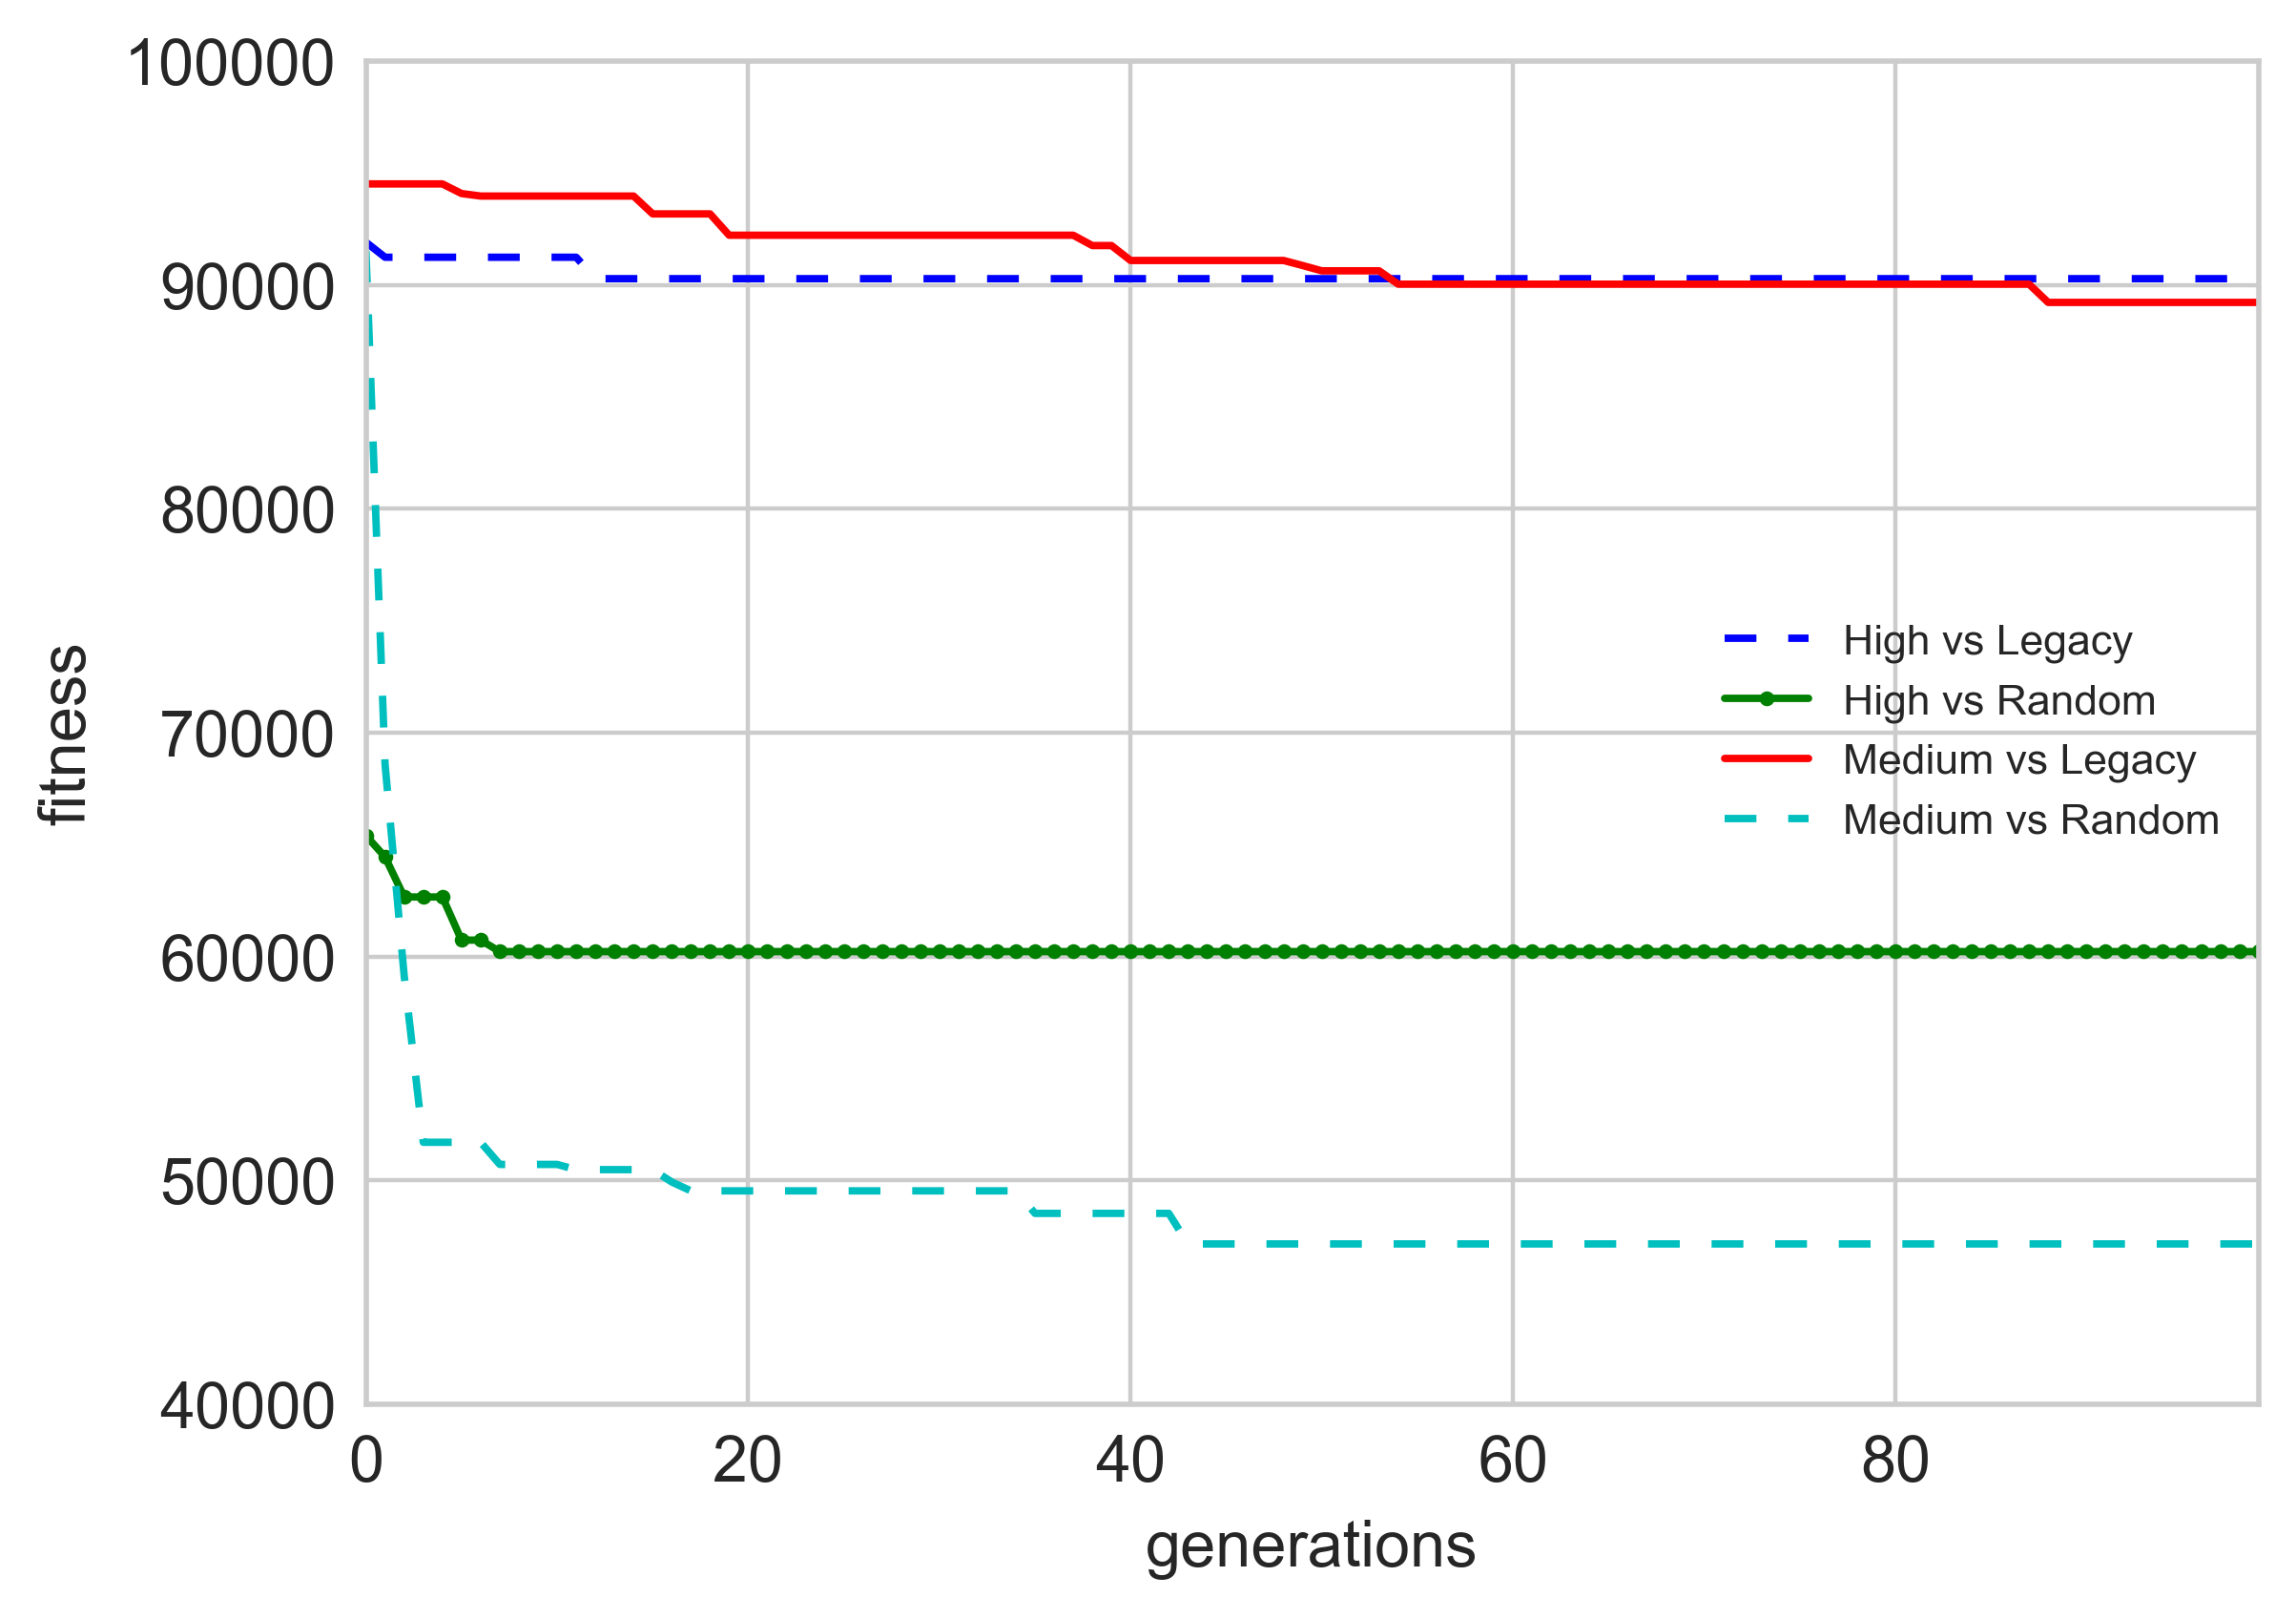
\includegraphics[width=1\textwidth]{so_fitness_bests}
    \caption{Objective fitness (Naive fitness).}
\end{figure}

%%%%%%%%%%%%%%%%%%%%%%%%%%%%%%%%%%%%%%%%%%
%
\section{Multi-objective optimization}
\label{sec:sec3}
%
%%%%%%%%%%%%%%%%%%%%%%%%%%%%%%%%%%%%%%%%%%

\subsection{Definition}

Multi-objective optimization arises when a single objective may not adequately represent the problem being faced, so modelling it with several objectives is preferred. Multi-objective optimization is therefore
\begin{equation}
\begin{aligned}
f_i(X) | i = 1,...,n
\end{aligned}
\end{equation}
where $n$ is the number of objectives and $f_i$ is the $ith$ fitness function.

The difficulty of this kind of algorithm lies on determine which individual optimizes all objectives better. Normally, we call a solution the Pareto optimal if none of the objective functions can be improved in value without degrading some of the other objective values, and can be formulated like this.\cite{cervigon}
\begin{equation}
\begin{aligned}
f_i(y) f_i(x), (i=1,\cdots,n) f_i(y) < f_j(x)
\end{aligned}
\end{equation}

Exist a wide variety of methods when implementing a multi-objective algorithm. The easiest consists in creating a fitness function which is a linear combination of all other functions to optimize.
\begin{equation}
\begin{aligned}
f(x) = \theta_1f_1(x) +\theta_2f_2(x) +\cdots+\theta_nf_n(x)
\end{aligned}
\end{equation}
where $\theta_i$ are coefficients used to balance the weight of each function. The main problem concerns the difficulty to find the adequate weights.

A very popular approach is the one called \textit{NSGA-II}\cite{nsgapaper}, which delivers very good results. It is however too computationally expensive, especially for large populations.

\subsection{Why to apply it}
Using a single objective function that maximizes score, inevitably leads to bots that keep moving around a power pill until one or more ghosts approach. Then \paco eats the power pill and proceed to eat as many ghosts as possible, making good profit out of it.

This strategy only works when there are still power pills available. With no power pills left, \paco keeps rambling until a ghost eats it and the game is over. So it is clear that we need to counterbalance ghost score to pass to next level.

Instead of overcomplicating the objective function trying to fulfil several goals, we simply define several objective functions in charge of different desirable aspects of the bots.
{\color{red} DIRÍA QUE NECESITAMOS UN ARGUMENTO MÁS CONVINCENTE, CON PRUEBAS INCLUSO}

\begin{equation}
f_2 = 100 - \text{last level reached}
% caption: levels completed
\end{equation}

We can even define the vanilla score function without the ghost multiplier.
\begin{equation}
\begin{split}
f_3 = 100000 - & (\text{pills eaten} \times \text{pill score} \\
& + \text{power pills eaten} \times \text{power pill score} \\
& + \text{ghosts eaten} \times \text{ghost score}) \\
% caption: no ghosts multiplier
\end{split}
\end{equation}

With a combination like $F = [f_2, f_3]$ a working multi-objective function can be created.

\subsection{Experiments and results}
{\color{red} Pruebas en curso}

{\color{red}ANTONIO: comparar el multiobjetivo con los resultados del apartado anterior. Al menos se pasará más niveles, aunque consiga peor puntuación...}

% Please add the following required packages to your document preamble:
% \usepackage{multirow}
\begin{table}[H]
\centering
\caption{\paco vs Ghost controllers comparison including Multi-Objetive}
\label{my-label}
\begin{tabular}{|l|c|r|r|r|r|r|r|r|r|r|}
\hline
\multicolumn{1}{|c|}{\multirow{2}{*}{\textbf{Pac-Man bot}}} & \multirow{2}{*}{\textbf{Ghosts bot}} & \multicolumn{3}{c|}{\textbf{score}} & \multicolumn{3}{c|}{\textbf{level}} & \multicolumn{3}{c|}{\textbf{time}} \\ \cline{3-11} 
\multicolumn{1}{|c|}{} &  & \multicolumn{1}{c|}{\textbf{max}} & \multicolumn{1}{c|}{\textbf{avg}} & \multicolumn{1}{c|}{\textbf{std}} & \multicolumn{1}{c|}{\textbf{max}} & \multicolumn{1}{c|}{\textbf{avg}} & \multicolumn{1}{c|}{\textbf{std}} & \multicolumn{1}{c|}{\textbf{max}} & \multicolumn{1}{c|}{\textbf{avg}} & \multicolumn{1}{c|}{\textbf{std}} \\ \hline
RandomNonRev & \multirow{8}{*}{Random} & 4840 & 1820 & 672 & 1 & 0.007 & 0.083 & 4831 & 1751 & 701.5 \\ \cline{1-1} \cline{3-11} 
Random &  & 1380 & 501 & 213 & 1 & 0.036 & 0.186 & 5635 & 1943 & 887.5 \\ \cline{1-1} \cline{3-11} 
NearestPill &  & 18910 & 4471 & 2654 & 5 & 1 & 0.9 & 7216 & 1795 & 1018 \\ \cline{1-1} \cline{3-11} 
NearestPillVS &  & 16060 & 4530 & 2674 & 5 & 1.1 & 0.9 & 6312 & 1823 & 1050 \\ \cline{1-1} \cline{3-11} 
\textbf{Medium-level} &  & \textbf{64600} & \textbf{48558} & \textbf{10780} & \textbf{18} & \textbf{15} & \textbf{3.4} & \textbf{24000} & \textbf{21579} & \textbf{4470} \\ \cline{1-1} \cline{3-11} 
\textbf{Medium-level (MO)} &  & \textbf{62050} & \textbf{46922} & \textbf{1243} & \textbf{18} & \textbf{15} & \textbf{4} & \textbf{24000} & \textbf{20868} & \textbf{5094.5} \\ \cline{1-1} \cline{3-11} 
\textbf{High-level} &  & \textbf{55480} & \textbf{32704} & \textbf{13237} & \textbf{18} & \textbf{10.4} & \textbf{4.3} & \textbf{24000} & \textbf{17457} & \textbf{6784} \\ \cline{1-1} \cline{3-11} 
\textbf{High-level (MO)} &  & \textbf{57370} & \textbf{32441} & \textbf{12712} & \textbf{17} & \textbf{10} & \textbf{4.1} & \textbf{24000} & \textbf{17536} & \textbf{6604.7} \\ \hline
RandomNonRev & \multirow{8}{*}{Legacy} & 6040 & 1502 & 792 & 0 & 0 & 0 & 3182 & 903 & 367.7 \\ \cline{1-1} \cline{3-11} 
Random &  & 1840 & 197 & 107 & 0 & 0 & 0 & 877 & 465 & 61.3 \\ \cline{1-1} \cline{3-11} 
NearestPill &  & 7190 & 3531 & 638 & 1 & 0.4 & 0.5 & 1881 & 1152 & 143.7 \\ \cline{1-1} \cline{3-11} 
NearestPillVS &  & 11100 & 3533 & 731 & 2 & 0.4 & 0.5 & 3218 & 1152 & 163 \\ \cline{1-1} \cline{3-11} 
\textbf{Medium-level} &  & \textbf{15960} & \textbf{6358} & \textbf{2883} & \textbf{3} & \textbf{0.9} & \textbf{0.7} & \textbf{4973} & \textbf{1916} & \textbf{730} \\ \cline{1-1} \cline{3-11} 
\textbf{Medium-level (MO)} &  & \textbf{10440} & \textbf{3273} & \textbf{852} & \textbf{2} & \textbf{0.8} & \textbf{0.4} & \textbf{5245} & \textbf{1551} & \textbf{309} \\ \cline{1-1} \cline{3-11} 
\textbf{High-level} &  & \textbf{20040} & \textbf{5972} & \textbf{2832} & \textbf{4} & \textbf{1} & \textbf{0.6} & \textbf{8364} & \textbf{2026} & \textbf{1020} \\ \cline{1-1} \cline{3-11} 
\textbf{High-level (MO)} &  & \textbf{20040} & \textbf{5972} & \textbf{2832} & \textbf{4} & \textbf{1} & \textbf{0.6} & \textbf{8364} & \textbf{2026} & \textbf{1020} \\ \hline
\end{tabular}
\end{table}

\begin{figure}[H]
    \centering
    \begin{subfigure}[b]{\textwidth}
        \includegraphics[width=1\textwidth]{mo_fitness_obj2_bests}
        \caption{Naive fitness}
        \label{fig:mo_fitness1}
    \end{subfigure}
    ~ %add desired spacing between images, e. g. ~, \quad, \qquad, \hfill etc. 
      %(or a blank line to force the subfigure onto a new line)
    \begin{subfigure}[b]{\textwidth}
        \includegraphics[width=1\textwidth]{mo_fitness_obj1_bests}
        \caption{Number of levels completed fitness}
        \label{fig:mo_fitness1}
    \end{subfigure}
    \caption{Objective fitnesses}\label{fig:Objective evolution}
\end{figure}

\subsubsection{(Learned strategies)}
{\color{red} en curso.}

%%%%%%%%%%%%%%%%%%%%%%%%%%%%%%%%%%%%%%%%%%
%
\section{Conclusions}
\label{sec:conclusions}
%
%%%%%%%%%%%%%%%%%%%%%%%%%%%%%%%%%%%%%%%%%%


Dejar para el final

Añadir al final la URL al repositorio de GitHub
\url{https://github.com/hecoding/Pac-Man}

\bibliographystyle{plain}
\bibliography{references.bib}

\end{document}
